\chapter{Appendix}

\section{Index Search Data Structures}\label{app:IndexSearchDataStructures}

\begin{itemize}
  \item \textbf{seq}: The sequence of characters as read from the FASTA/FASTQ files. May contain any character in the ASCII list. It is basically a string of characters, that may contain items other than our four characters alphabet of $ACGT$. This may contain characters from different sequences, too. The parser keeps reading the list of files for new characters until the maximum number of characters it should read in a single batch is read, or until the maximum number of different sequences it can span is reached, or until the end of the files is reached.
  \item \textbf{chars\_before\_newline}: An array of the number of characters which must be processed before the next character is considered to originate from a new sequence. For example, given the array $[4, 10, \infty]$, then it is known that the first four characters in \textbf{seq} are from the first sequence, the next six characters are from the second sequence, whereas the rest of the characters are from the third sequence. Note that this does not mean that the first sequence is four characters long, nor does the algorithm know how long the last sequence is, since a sequence may be split between two batches, for load balancing, hence why this array is important. A part of the first sequence may have been part of the previous batch, or could have spanned more than two batches if it was super long, whereas the third sequence may have been too large to fit in this batch, so the next batch will need to process the next part of it.
  \item \textbf{newlines\_before\_newfile}: Similar to what \textbf{chars\_before\_newline} is for characters, but instead this works for sequences. Thus, given the array $[3, 4, \infty]$, it means that in the input for this batch, the sequences came from three files, and the first three sequences came from the first file, the fourth sequence came from the second file, whereas the last sequence came from the third file. Note that this does not mean that the first file is three sequences long, nor does the algorithm know how large the third file is, since a file may be split between two batches, for load balancing, hence why this array is important.
  \item \textbf{bits}: Using a full byte for each character is wasteful when the alphabet is only four characters. Thus it is possible to convert $ACGT$ to $00, 01, 10, 11$ respectively, and this array of u64s contains the bitpacked characters. Thus, a single u64 can hold 32 characters, so to hold more than 32 characters per batch, an array of u64s is used, which is what this array is used for.
  \item \textbf{invalid\_chars}: Sometimes the sequences in the FASTQ file, and therefore contents of the \textbf{seq} string, may contain characters other than $ACGT$. The $k$-mers which contain these characters are invalid for this use case, and should thus be marked as such. Therefore, this array of booleans contains the same amount of elements as \textbf{seq}, and contains a 0 if the corresponding character at the same index in \textbf{seq} is part of the $ACGT$ alphabet, otherwise it will contain 1. For example, given \textbf{seq} \textit{ACNBGT}, this array will contain $[0, 0, 1, 1, 0, 0]$, as characters $N$ and $B$ are invalid. For the implementation in this algorithm, an array of chars is used rather than booleans, as this data type was found to be slightly faster, since the CPU does not need to perform any unnecessary bit shifts.
  \item \textbf{positions}: There are fewer $k$-mers than there are characters. If there are 10 characters in a sequence and $k=7$, then there are 4 $k$-mers in this sequence, and the first character of these $k$-mers would be the characters at indexes 0, 1, 2, and 3. These indexes are the positions array. When there are multiple sequences, so if the algorithm is given two sequences, each 10 characters long, and they would be in the same batch, that is, \textbf{seq} is of size 20, then the positions array would be $[0, 1, 2, 3, 10, 11, 12, 13]$, as the $k$-mers for the second sequence start later, at index 10.
\end{itemize}

\section{Color Search Data Structures}\label{app:ColorSearchDataStructures}

\begin{itemize}
  \item \textbf{warped\_indexes}: The indexes of colored sequences in a u64 array. When the indexes are read from the file, they are put into this array, which will later be put on the GPU. The goal is such that each thread in the GPU handles a single index, and a single warp handles indexes from a single sequence. This means that a warp can not have indexes from two different sequences. However, the indexes of a sequence are allowed to be spread over multiple warps. Thus, the indexes are loaded until the end of a sequence, and then padding is inserted for the rest of the warp, so that the first index of the next sequence will be loaded at the first position of the next warp. So, given two sequences with indexes $[45, 21, 32, 25, 21]$ and $[23, 22, 93, 34]$, and given a warp size of 4, then this array would contain $[45, 21, 32, 25, 21, -1, -1, -1, 23, 22, 93, 34]$, where the $-1$ represents padding, the first eight indexes are of the first and second warp, which contain the indexes of the first sequence plus padding, and the last four indexes are of the third warp which contain the indexes of the second sequence. Since the second sequence has an index count which is a multiple of the warp size, there is no need for padding.
  \item \textbf{warp\_intervals}: The indexes are all in a single array, inside the \textbf{warped\_indexes}. Therefore, there needs to be some mechanism to tell which indexes come from the first sequence, and which indexes come from the second sequence. This array provides that mechanism, such that it tells at which warp index a new sequence starts. Given the previous example, this array would contain $0, 2, 3$. The last value exists for convenience, and it allows the programmer to know how many warps in total are loaded with indexes.
  \item \textbf{found\_idxs}: When $\tau$ is not equal to 1, it is necessary to check if enough indexes of the sequence actually belong to the DBG. This array takes a count of how many indexes of each sequence belong to the DBG. Note that a colored sequence has this value equal to at least 1. Therefore, this array has a single entry per sequence.
  \item \textbf{not\_found\_idxs}: When $\tau$ is not equal to 1, it is thus also necessary to know how many indexes of the sequence are not found in the DBG. This array takes count of those. Thus it also has one entry per sequence.
  \item \textbf{invalid\_idxs}: In the implementation provided in this thesis, a distinction is made between indexes which are not found and those which are invalid, hence this array contains a count of how many invalid indexes existed for each sequence.
  \itm \textbf{results}: This array contains the colors of the colored sequences, after they are post processed in the GPU. The format of this array takes a lot of space, such that if there are $n$ colors in total, and $m$ colored sequence, this array takes $nm$ spaces.
  \item \textbf{colored\_seq\_id}: Since not all sequences have entries in \textbf{warped\_indexes}, the algorithm needs to know where the colors of a colored sequence are after post processing. It can know if a sequence is colored or not by simply checking if the \textbf{found\_idxs} for this sequence is greater than zero. If the sequences are accessed serially, then it would be easy to know which colors belong to which sequence, simply by keeping a counter, and after encountering a colored sequence, the counter would be increased by one. However, if the results and the sequences are to be accessed in parallel, then this array allows the algorithm to know where to look for the \textbf{results} of this sequence. Thus, this array also has an entry per sequence, however, the blank sequences ignore this value as they do not have any entries in the \textbf{results} array.
  \item \textbf{seqs\_before\_newfile}: This is the same as for the Index Search phase, it keeps track of how many sequences belong to the first file, how many for the second, etc.
\end{itemize}

\section{Components and Batches}\label{app:Batches}

\begin{figure}[h!]
  \centering
  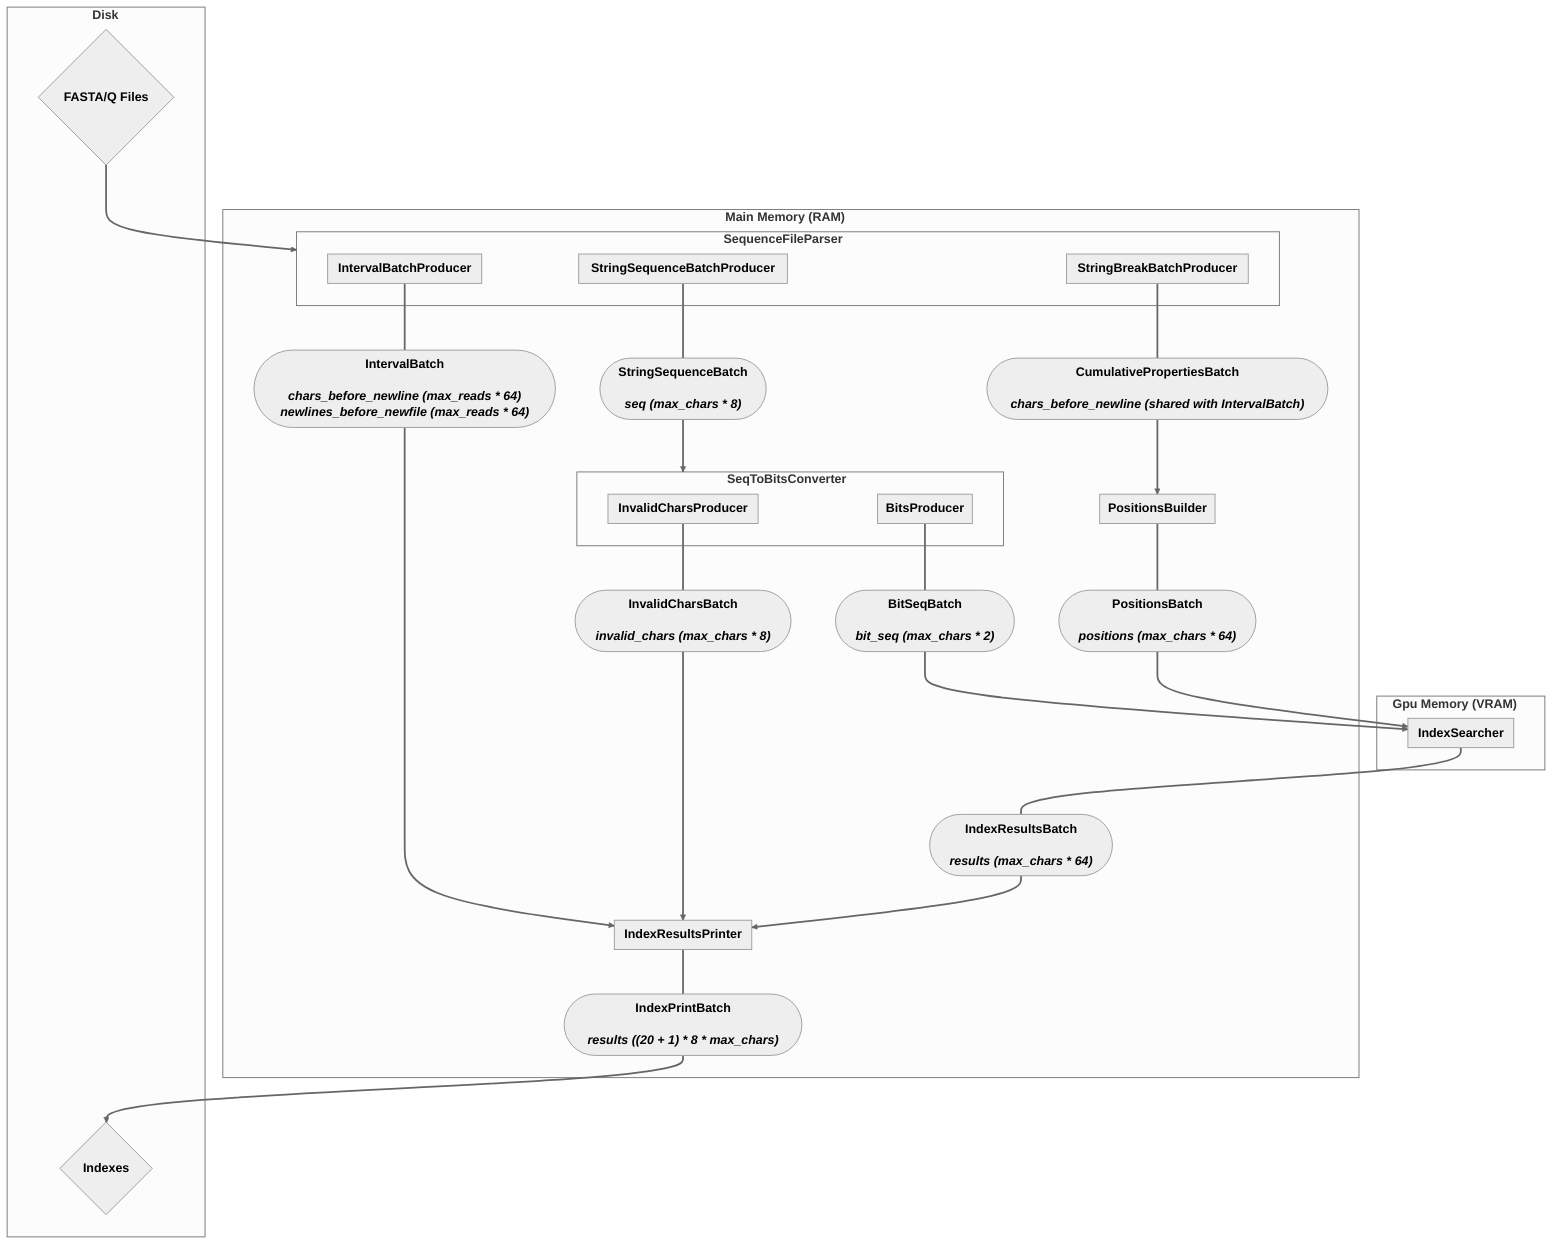
\includegraphics[width=\textwidth]{images/IndexBatches.png}
  \caption{The Index components and how their batches are shared between components. The amount of space that each batch uses is also listed below it, with the format of <variable>(<size taken>). These sizes are taken into consideration when reserving memory for each batch, by first deciding the maximum number of characters and then reserving memory accordingly. The diamond shapes represent items stored on disk, square shapes represent components, and items in the rectangle with curved sides are the batches.}\label{fig:IndexBatches}
\end{figure}


\begin{figure}[h!]
  \centering
  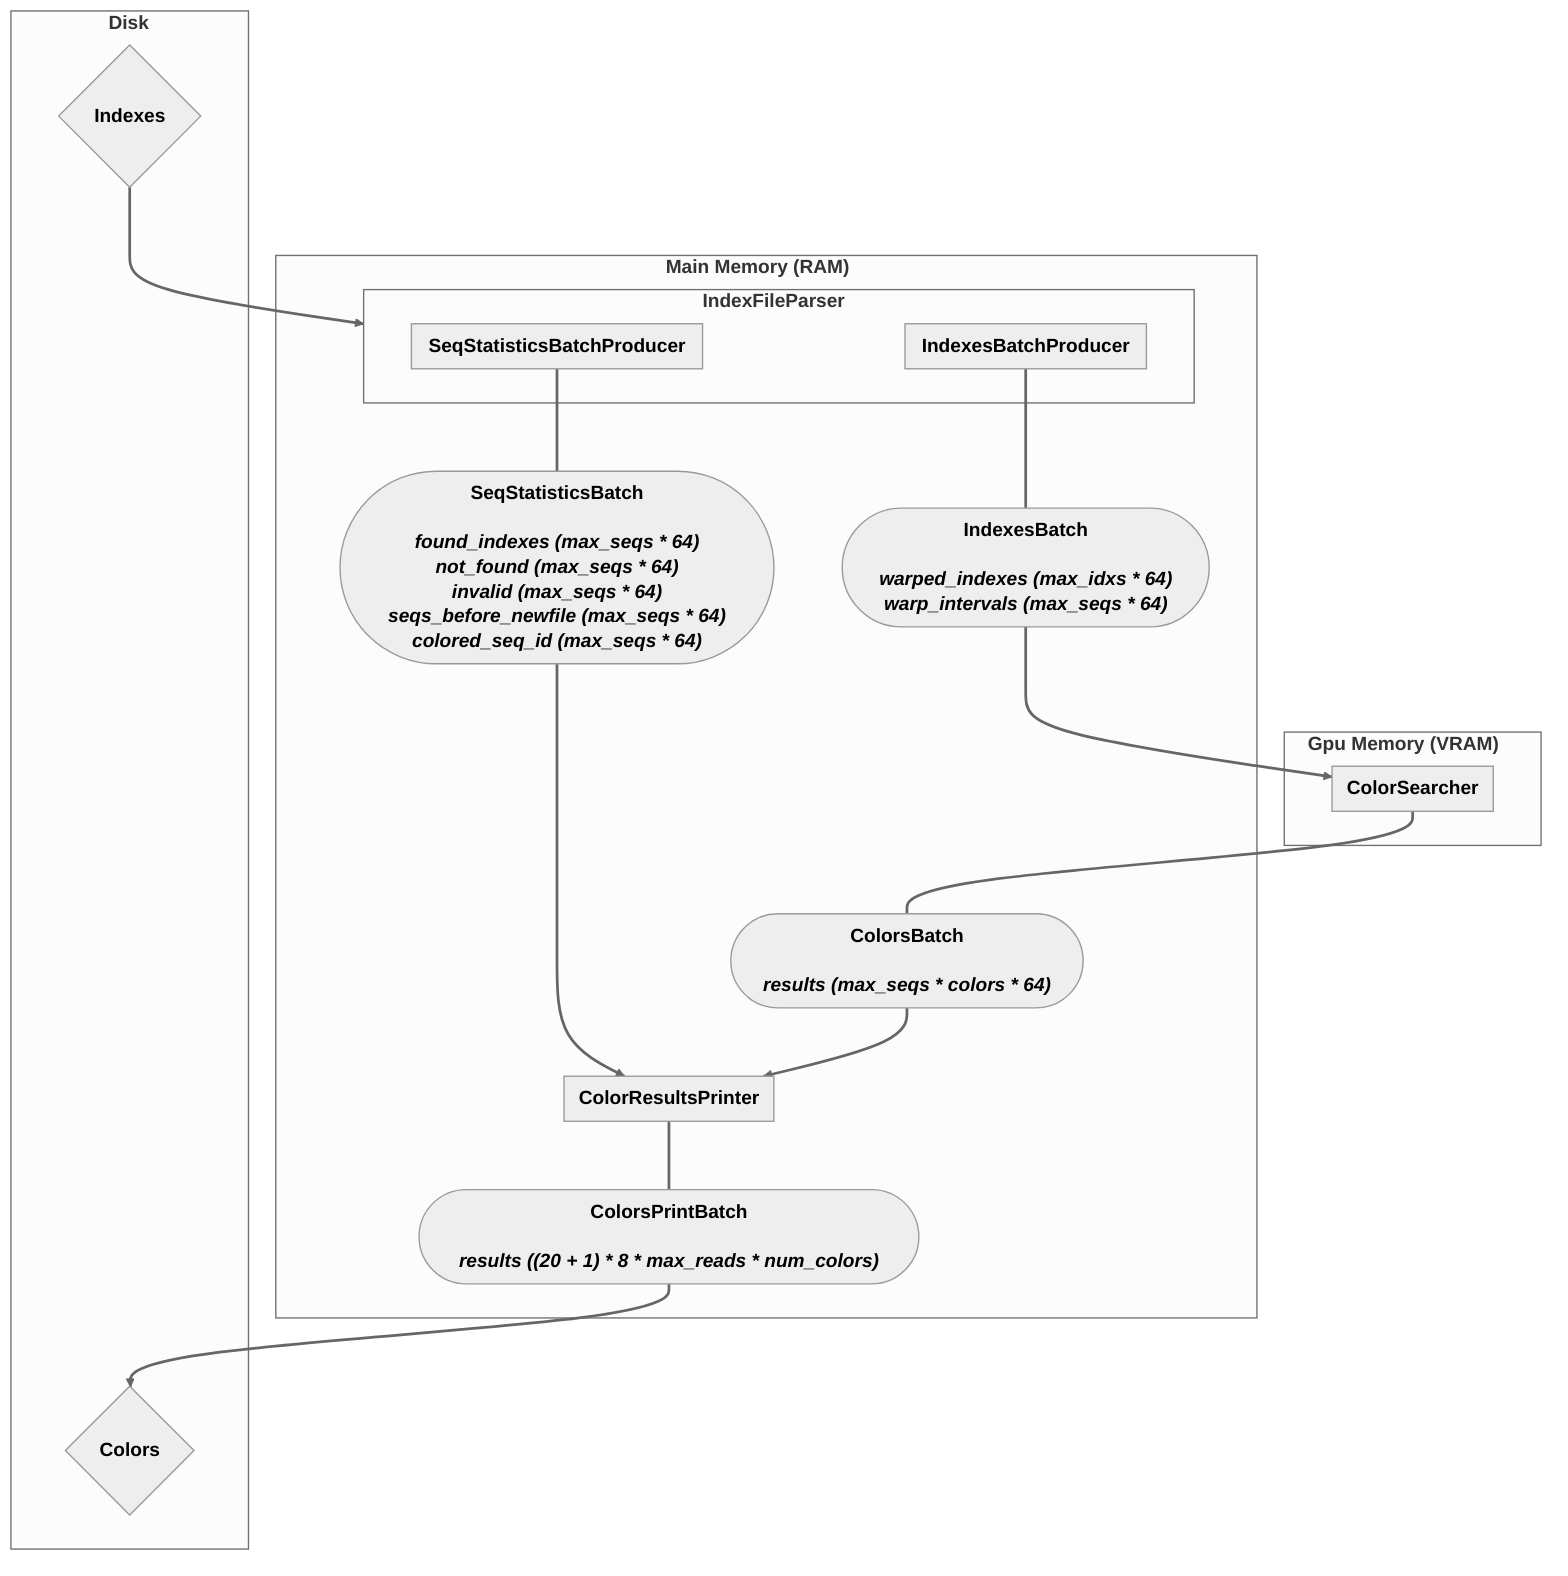
\includegraphics[width=\textwidth]{images/ColorBatches.png}
  \caption{The Colors components and how their batches are shared between components. The amount of space that each batch uses is also listed below it, with the format of <variable>(<size taken>). These sizes are taken into consideration when reserving memory for each batch, by first deciding the maximum number of characters and then reserving memory accordingly. The diamond shapes represent items stored on disk, square shapes represent components, and items in the rectangle with curved sides are the batches.}\label{fig:ColorBatches}
\end{figure}

\clearpage
\section{Dataset Filename List}\label{app:file_names}

\begin{footnotesize}
\begin{verbatim}
  ftp.sra.ebi.ac.uk/vol1/fastq/ERR340/004/ERR3404624/ERR3404624_2.fastq.gz
  ftp.sra.ebi.ac.uk/vol1/fastq/ERR340/005/ERR3404625/ERR3404625_1.fastq.gz
  ftp.sra.ebi.ac.uk/vol1/fastq/ERR340/005/ERR3404625/ERR3404625_2.fastq.gz
  ftp.sra.ebi.ac.uk/vol1/fastq/ERR340/006/ERR3404626/ERR3404626_1.fastq.gz
  ftp.sra.ebi.ac.uk/vol1/fastq/ERR340/006/ERR3404626/ERR3404626_2.fastq.gz
  ftp.sra.ebi.ac.uk/vol1/fastq/ERR340/007/ERR3404627/ERR3404627_1.fastq.gz
  ftp.sra.ebi.ac.uk/vol1/fastq/ERR340/007/ERR3404627/ERR3404627_2.fastq.gz
  ftp.sra.ebi.ac.uk/vol1/fastq/ERR340/008/ERR3404628/ERR3404628_1.fastq.gz
  ftp.sra.ebi.ac.uk/vol1/fastq/ERR340/008/ERR3404628/ERR3404628_2.fastq.gz
  ftp.sra.ebi.ac.uk/vol1/fastq/ERR340/009/ERR3404629/ERR3404629_1.fastq.gz
  ftp.sra.ebi.ac.uk/vol1/fastq/ERR340/009/ERR3404629/ERR3404629_2.fastq.gz
  ftp.sra.ebi.ac.uk/vol1/fastq/ERR340/000/ERR3404630/ERR3404630_1.fastq.gz
  ftp.sra.ebi.ac.uk/vol1/fastq/ERR340/000/ERR3404630/ERR3404630_2.fastq.gz
  ftp.sra.ebi.ac.uk/vol1/fastq/ERR340/001/ERR3404631/ERR3404631_1.fastq.gz
  ftp.sra.ebi.ac.uk/vol1/fastq/ERR340/001/ERR3404631/ERR3404631_2.fastq.gz
  ftp.sra.ebi.ac.uk/vol1/fastq/ERR340/002/ERR3404632/ERR3404632_1.fastq.gz
  ftp.sra.ebi.ac.uk/vol1/fastq/ERR340/002/ERR3404632/ERR3404632_2.fastq.gz
  ftp.sra.ebi.ac.uk/vol1/fastq/ERR340/003/ERR3404633/ERR3404633_1.fastq.gz
  ftp.sra.ebi.ac.uk/vol1/fastq/ERR340/003/ERR3404633/ERR3404633_2.fastq.gz
  ftp.sra.ebi.ac.uk/vol1/fastq/ERR340/004/ERR3404634/ERR3404634_1.fastq.gz
  ftp.sra.ebi.ac.uk/vol1/fastq/ERR340/004/ERR3404634/ERR3404634_2.fastq.gz
  ftp.sra.ebi.ac.uk/vol1/fastq/ERR340/005/ERR3404635/ERR3404635_1.fastq.gz
  ftp.sra.ebi.ac.uk/vol1/fastq/ERR340/005/ERR3404635/ERR3404635_2.fastq.gz
  ftp.sra.ebi.ac.uk/vol1/fastq/ERR340/006/ERR3404636/ERR3404636_1.fastq.gz
\end{verbatim}
\end{footnotesize}

\clearpage
\section{Results Table Description}

In Chapter~\ref{ch:Results}, there are figures with timelines and a table underneath the timeline.
These bullet points give a description of what each component means.
When a bullet point is a sub-bullet of another item, it means that the parent item includes the time of the sub-bullet.

\subsubsection{Index Search}\label{app:IndexTableDescriptions}

\begin{itemize}
  \item \textbf{main}: The entire program from start to finish.
  \begin{itemize}
    \item \textbf{SBWTLoader}: The starting phase besides memory loading.
    \begin{itemize}
      \item \textbf{SBWTParserAndIndex}: Reading the SBWT from disk, building the poppy, and transferring to GPU.
      \begin{itemize}
        \item \textbf{SBWTReadAndPoppy}: Same as parent but without the construction of the class which does the work.
      \end{itemize}
      \item \textbf{SBWTGpuTransfer}: Copying the SBWT to GPU.
      \item \textbf{Presearcher}: The construction of the presearch map.
      \begin{itemize}
        \item \textbf{PresearchFunction}: Same as parent but without construction of objects such as the allocation in GPU memory.
      \end{itemize}
    \end{itemize}
    \item \textbf{MemoryAllocator}: The allocation of memory for each of the components, some of which is pinned memory.
    \begin{itemize}
      \item \textbf{SequenceFileParserAllocator}: Memory allocation for the SequenceFileParser.
      \item \textbf{SeqToBitsConverterAllocator}: Memory allocation for the SeqToBitsConverter.
      \item \textbf{PositionsBuilderAllocator}: Memory allocation for the PositionsBuilder.
      \item \textbf{SearcherAllocator}: Memory allocation for the Searcher, on both CPU and GPU.
      \item \textbf{ResultsPrinterAllocator}: Memory allocation for the ResultsPrinter.
    \end{itemize}
    \item \textbf{Querier}: The query time, which is the time taken by the program without the startup.
    \begin{itemize}
      \item \textbf{SequenceFileParser}: The component which reads the sequence FASTA or FASTQ files.
      \item \textbf{PositionsBuilder}: The component which builds the positions.
      \item \textbf{SeqToBitsConverter}: The component which bit-packs sequences.
      \item \textbf{Searcher}: The component which searches for the indexes given the necessary items on the GPU.
      \begin{itemize}
        \item \textbf{SearcherCopyToGpu}: Copying the positions and bit-packed sequences to GPU.
        \item \textbf{SearcherSearch}: The kernel itself.
        \item \textbf{SearcherCopyFromGpu}: Copying the results back to CPU.
      \end{itemize}
    \end{itemize}
    \item \textbf{ResultsPrinter}: Printing the results to disk.
  \end{itemize}
\end{itemize}

\subsubsection{Color Search}

\begin{itemize}
  \item \textbf{main}: The entire program from start to finish.
  \begin{itemize}
    \item \textbf{ColorsLoader}: Reading the colors from disk and into the GPU.
    \item \textbf{MemoryAllocator}: The allocation of memory for each of the components, some of which is pinned memory.
    \begin{itemize}
      \item \textbf{IndexFileParserAllocator}: Memory allocation for the IndexFileParser.
      \item \textbf{SearcherAllocator}: Memory allocation for the Searcher, on both CPU and GPU.
      \item \textbf{ResultsPrinterAllocator}: Memory allocation for the ResultsPrinter.
    \end{itemize}
    \item \textbf{Querier}: The query time, which is the time taken by the program without the startup.
    \begin{itemize}
      \item \textbf{ContinuousIndexFileParser}: The component which reads the index files.
      \item \textbf{Searcher}: The component which searches for the colors and does post processing, given the necessary items on the GPU.
      \begin{itemize}
        \item \textbf{SearcherCopyToGpu1}: Copying the indexes to GPU.
        \item \textbf{SearcherSearch}: The kernel for searching.
        \item \textbf{SearcherCopyToGpu2}: Copying the warps intervals to GPU.
        \item \textbf{SearcherPostProcess}: The kernel for post processing.
        \item \textbf{SearcherCopyFromGpu}: Copying the results back to CPU.
      \end{itemize}
    \item \textbf{ResultsPrinter}: Printing the results to disk.
    \end{itemize}
  \end{itemize}
\end{itemize}
